\newpage
\section{Process perspective}
\subsection{CI/CD Pipeline}
We have set up our CI/CD pipeline through GitHub Actions consisting of a total of 4 (5 if we count Dependabot) different workflows that trigger throughout the development process. 

\subsubsection*{Autorelease} \label{sec:autorelease}
The autorelease workflow is triggered on push to main as long as there have been made changes to the application (changes to the src-folder). First, it creates a new release tag, using the semantic versioning scheme (Major, Minor, Patch)\footnote{https://interrupt.memfault.com/blog/release-versioning \cite{semanticVersioning}}. By default, it will bump the Patch version on merges to main but can be modified by writing \textit{\#major} or \textit{\#minor} in the commit message, which then will bump the respective number. When the tag has been created, a release with the version tag and auto-generated release notes will be made.

\subsubsection*{Continuous Deployment}

\begin{figure}[H]
  \centering
  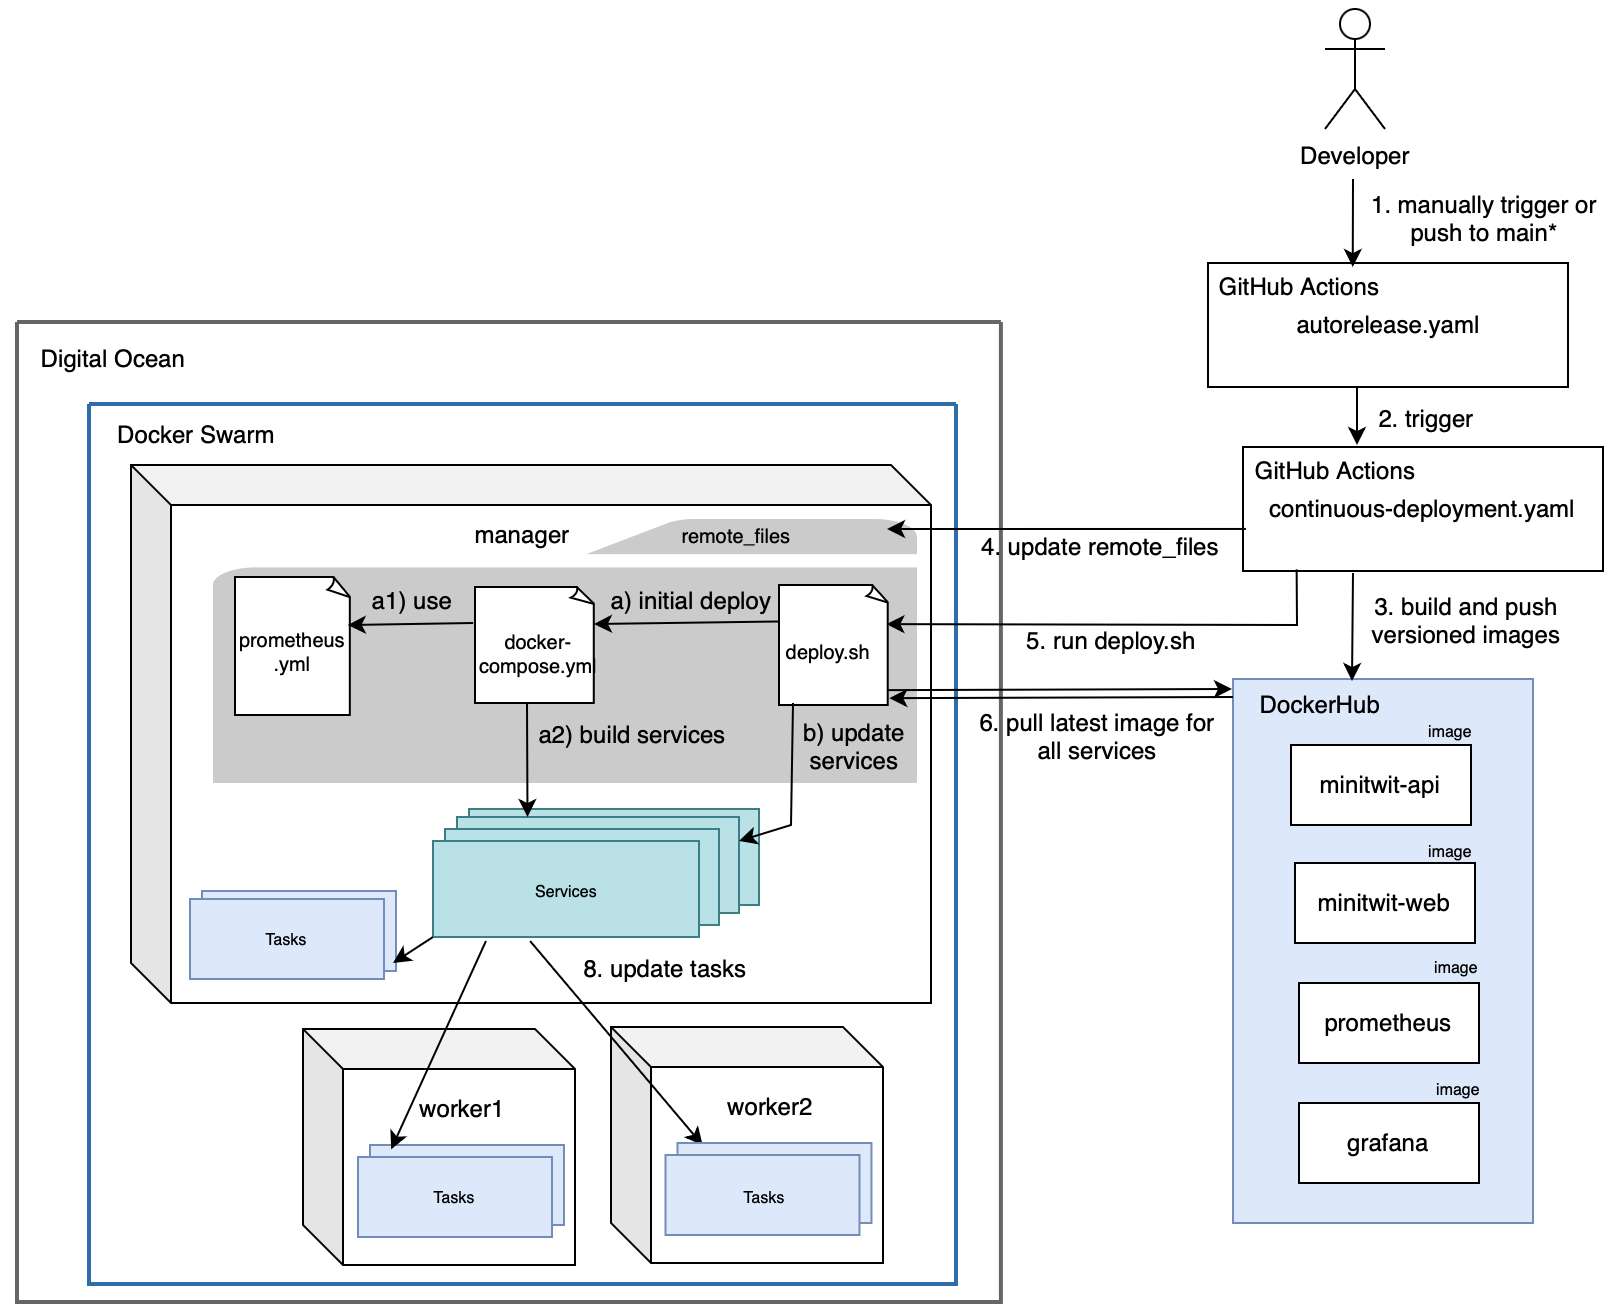
\includegraphics[width=0.75\textwidth]{Images/deployment.png}
  \caption{Deployment. Step 7a: These steps run only during the first deployment. Step 7b: For all subsequent deployments, this step is executed. The workflow does not depict the volumes for the services, for this level of detail see the figure of Docker Swarm.}
  \label{fig:dashboard}
\end{figure}

In addition to the steps shown above, the deployment process also tags the Docker images pushed to DockerHub with the version number created in the Autorelease (Section \ref{sec:autorelease}) as well as with a "latest" tag. This ensures that all versions of our application are preserved on DockerHub.

\subsubsection*{CodeQL}
The CodeQL workflow is triggered on pull requests to main and has a cron job every Wednesday at 16:20. It scans the code for vulnerabilities and quality issues by using a predefined set of queries. If issues are found, it provides detailed feedback, allowing us to address problems before merging changes into the main branch.
In hindsight, we should've decided between either running the workflow as either a cron job \textit{or} on pull requests. As it is now the cron job is irrelevant because the code gets checked every time before merged into main.

\subsubsection*{Linter}
The linter workflow is triggered on all pull requests and can be triggered manually also. It runs a super-linter for C\#, GitHub Actions, and Dockerfile, that checks for code quality and best practices throughout all the files in the codebase.

\subsubsection*{Dependabot}
The Dependabot workflow runs weekly, where it checks for updates throughout the codebase and create pull requests when updates are needed. Also to minimize bot spam every week, every Nuget update is getting grouped into one single pull request.


\subsection{Monitoring} %Skal rettes til og koges lidt ned
For the monitoring of our MiniTwit project, we utilize Prometheus and Grafana to store and visualize custom metrics from our system. Prometheus efficiently pulls data from various components and stores it as metrics, such as the current number of registered users and the rate of errors per second/minute. Grafana serves as our visualization tool, providing a range of customizable options for creating dashboards that offer a quick overview of the system's current status. \\

At the top section of our Grafana dashboard, we monitor the real-time status of the API and Web service. This includes tracking HTTP Requests per second and monitoring error codes. We also monitor the average CPU usage for the minitwit-api- and minitwit-web-services. Additionally, we track average page load times and API response times for various POST requests. The cumulative count of HTTP requests received provides insights into system usage over time, while error response codes highlight areas needing optimization. A pie chart summarizes the distribution of HTTP actions, offering a clear view of user interaction trends. This monitoring setup enables timely identification and resolution of potential issues, ensuring the project's health and performance.
\begin{figure}[H]
  \centering
  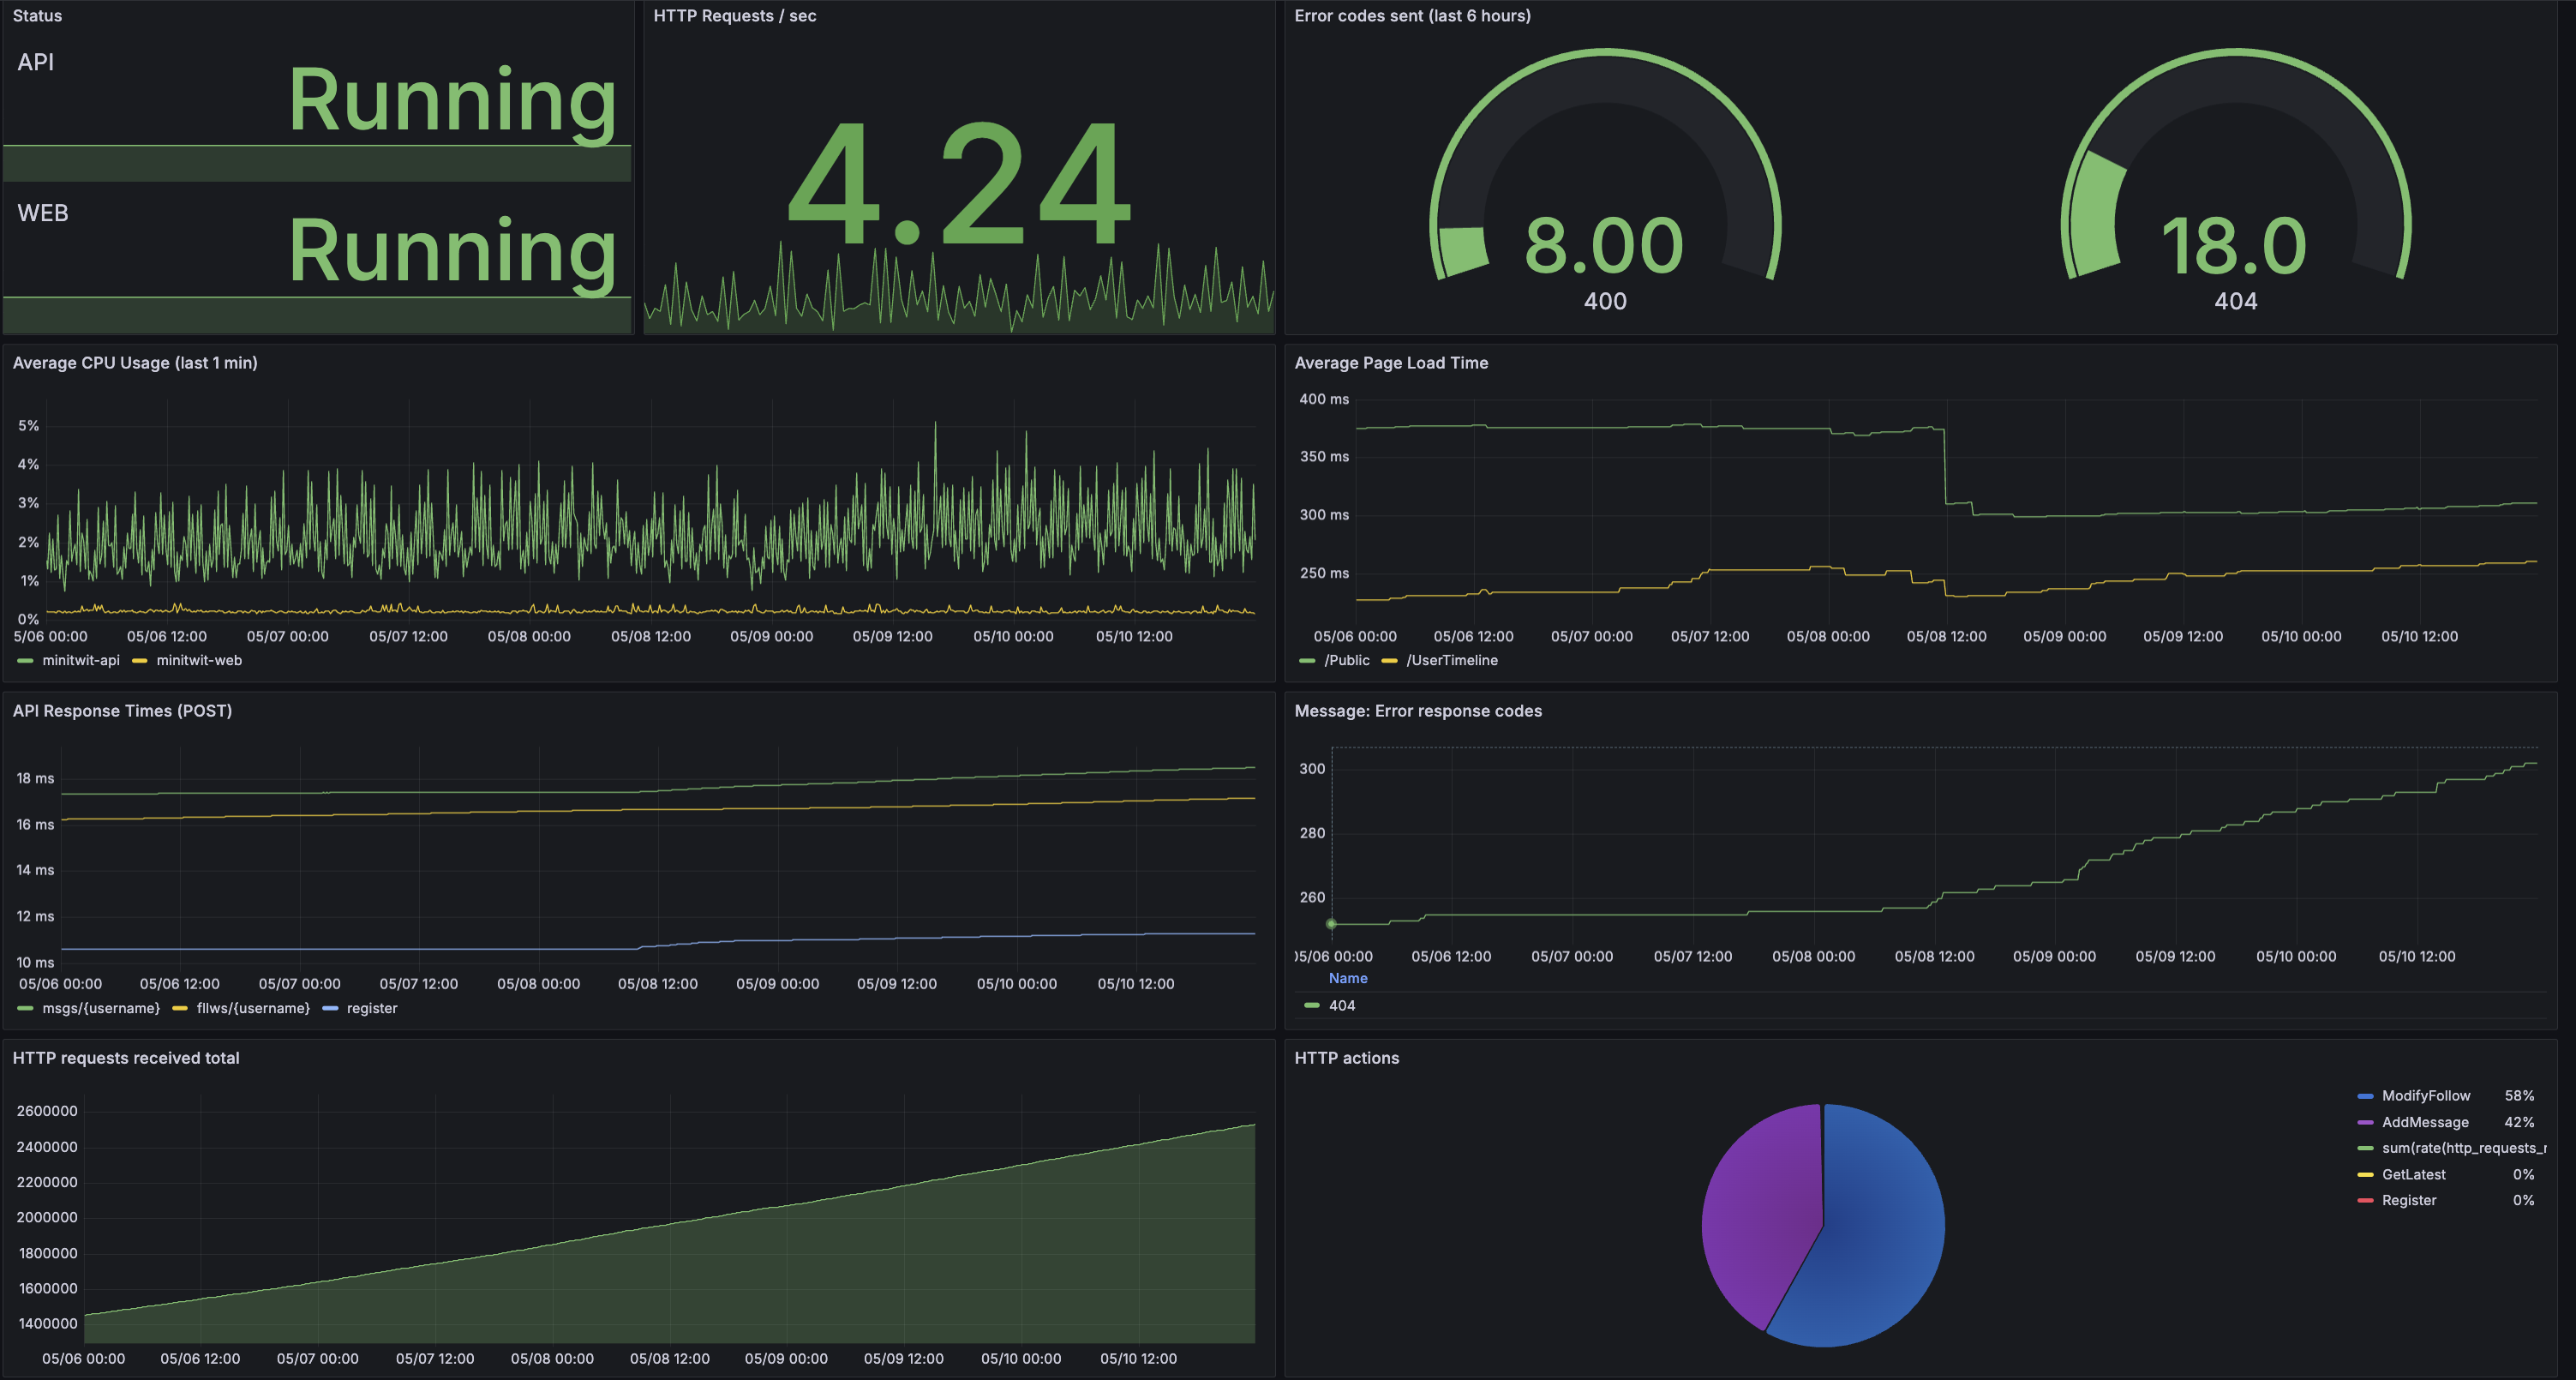
\includegraphics[width=\textwidth]{Images/Dashboard.png}
  \caption{Dashboard monitoring}
  \label{fig:dashboard}
\end{figure}

\subsection{Logging}
Logging for the application in production has not been set up yet, due to difficulties in implementing it. Read more about that in the lessons section \ref{lessons:logging}. The intended approach was to implement the ELK stack (Elasticsearch, Logstash, and Kibana), which are open-source tools designed to help us establish an easy-to-manage platform for logging, with the ability to modify and customize visuals as needed. The intended use of the different tools in the stack is as follows:
\begin{itemize}
    \item \textit{ElasticSearch} is an efficient search and analysis engine designed to handle the large text data generated by the logs.
    \item \textit{Logstash} is intended to aggregate and collect logs throughout the codebase.
    \item \textit{Kibana} utilizes the Elasticsearch indexes, search, and analysis capabilities to create visualizations of the data.
\end{itemize}

\subsection{Security}
In the Security and Risk analysis (see Appendix \ref{appendix:security_and_risk}) we have identified a variety of possible security issues. The identified risks highlight valid concerns and several safeguards could be implemented to enhance the application's security posture. Here are some potential changes that could be made:
\begin{itemize}
    \item Implementing rate limiting and input validation mechanisms would mitigate DDoS attacks and injection vulnerabilities.
    \item Securing cookies with the \verb|Secure| and \verb|HttpOnly| flags, along with robust authentication and authorization measures, would protect against unauthorized access and cookie manipulation.
    \item Running containers as a non-root user and securing database connections would reduce the impact of potential container escapes or data breaches.
    \item Implementing CAPTCHA/reCAPTCHA would protect us against bot spam.
\end{itemize} 

\subsection{Strategy for Scaling \& Upgrades}
\subsubsection*{Load balancing - Docker Swarm}
In our deployment of the MiniTwit application, we employ Docker Swarm to ensure high availability and efficient distribution of workloads across our infrastructure. Docker Swarm is a native clustering and orchestration tool for Docker containers, which allows us to manage a cluster of Docker nodes as a single system. By leveraging Docker Swarm, we can automatically distribute our services across multiple nodes, providing load balancing, fault tolerance, and scalability. \\

Our Docker Compose file on the manager droplet (remote\_files/docker-compose.yml) sets up the necessary services, networks, and volumes. We utilize external volumes to persist data for Prometheus and Grafana. \\

When defining the services, we use the update strategy \texttt{start-first}, which ensures that new instances are started before old ones are stopped during updates, minimizing downtime. \\

We use placement preferences and constraints, to ensure that exactly one instance of both the web and API service runs on each worker. \\

\begin{figure}[H]
  \centering
  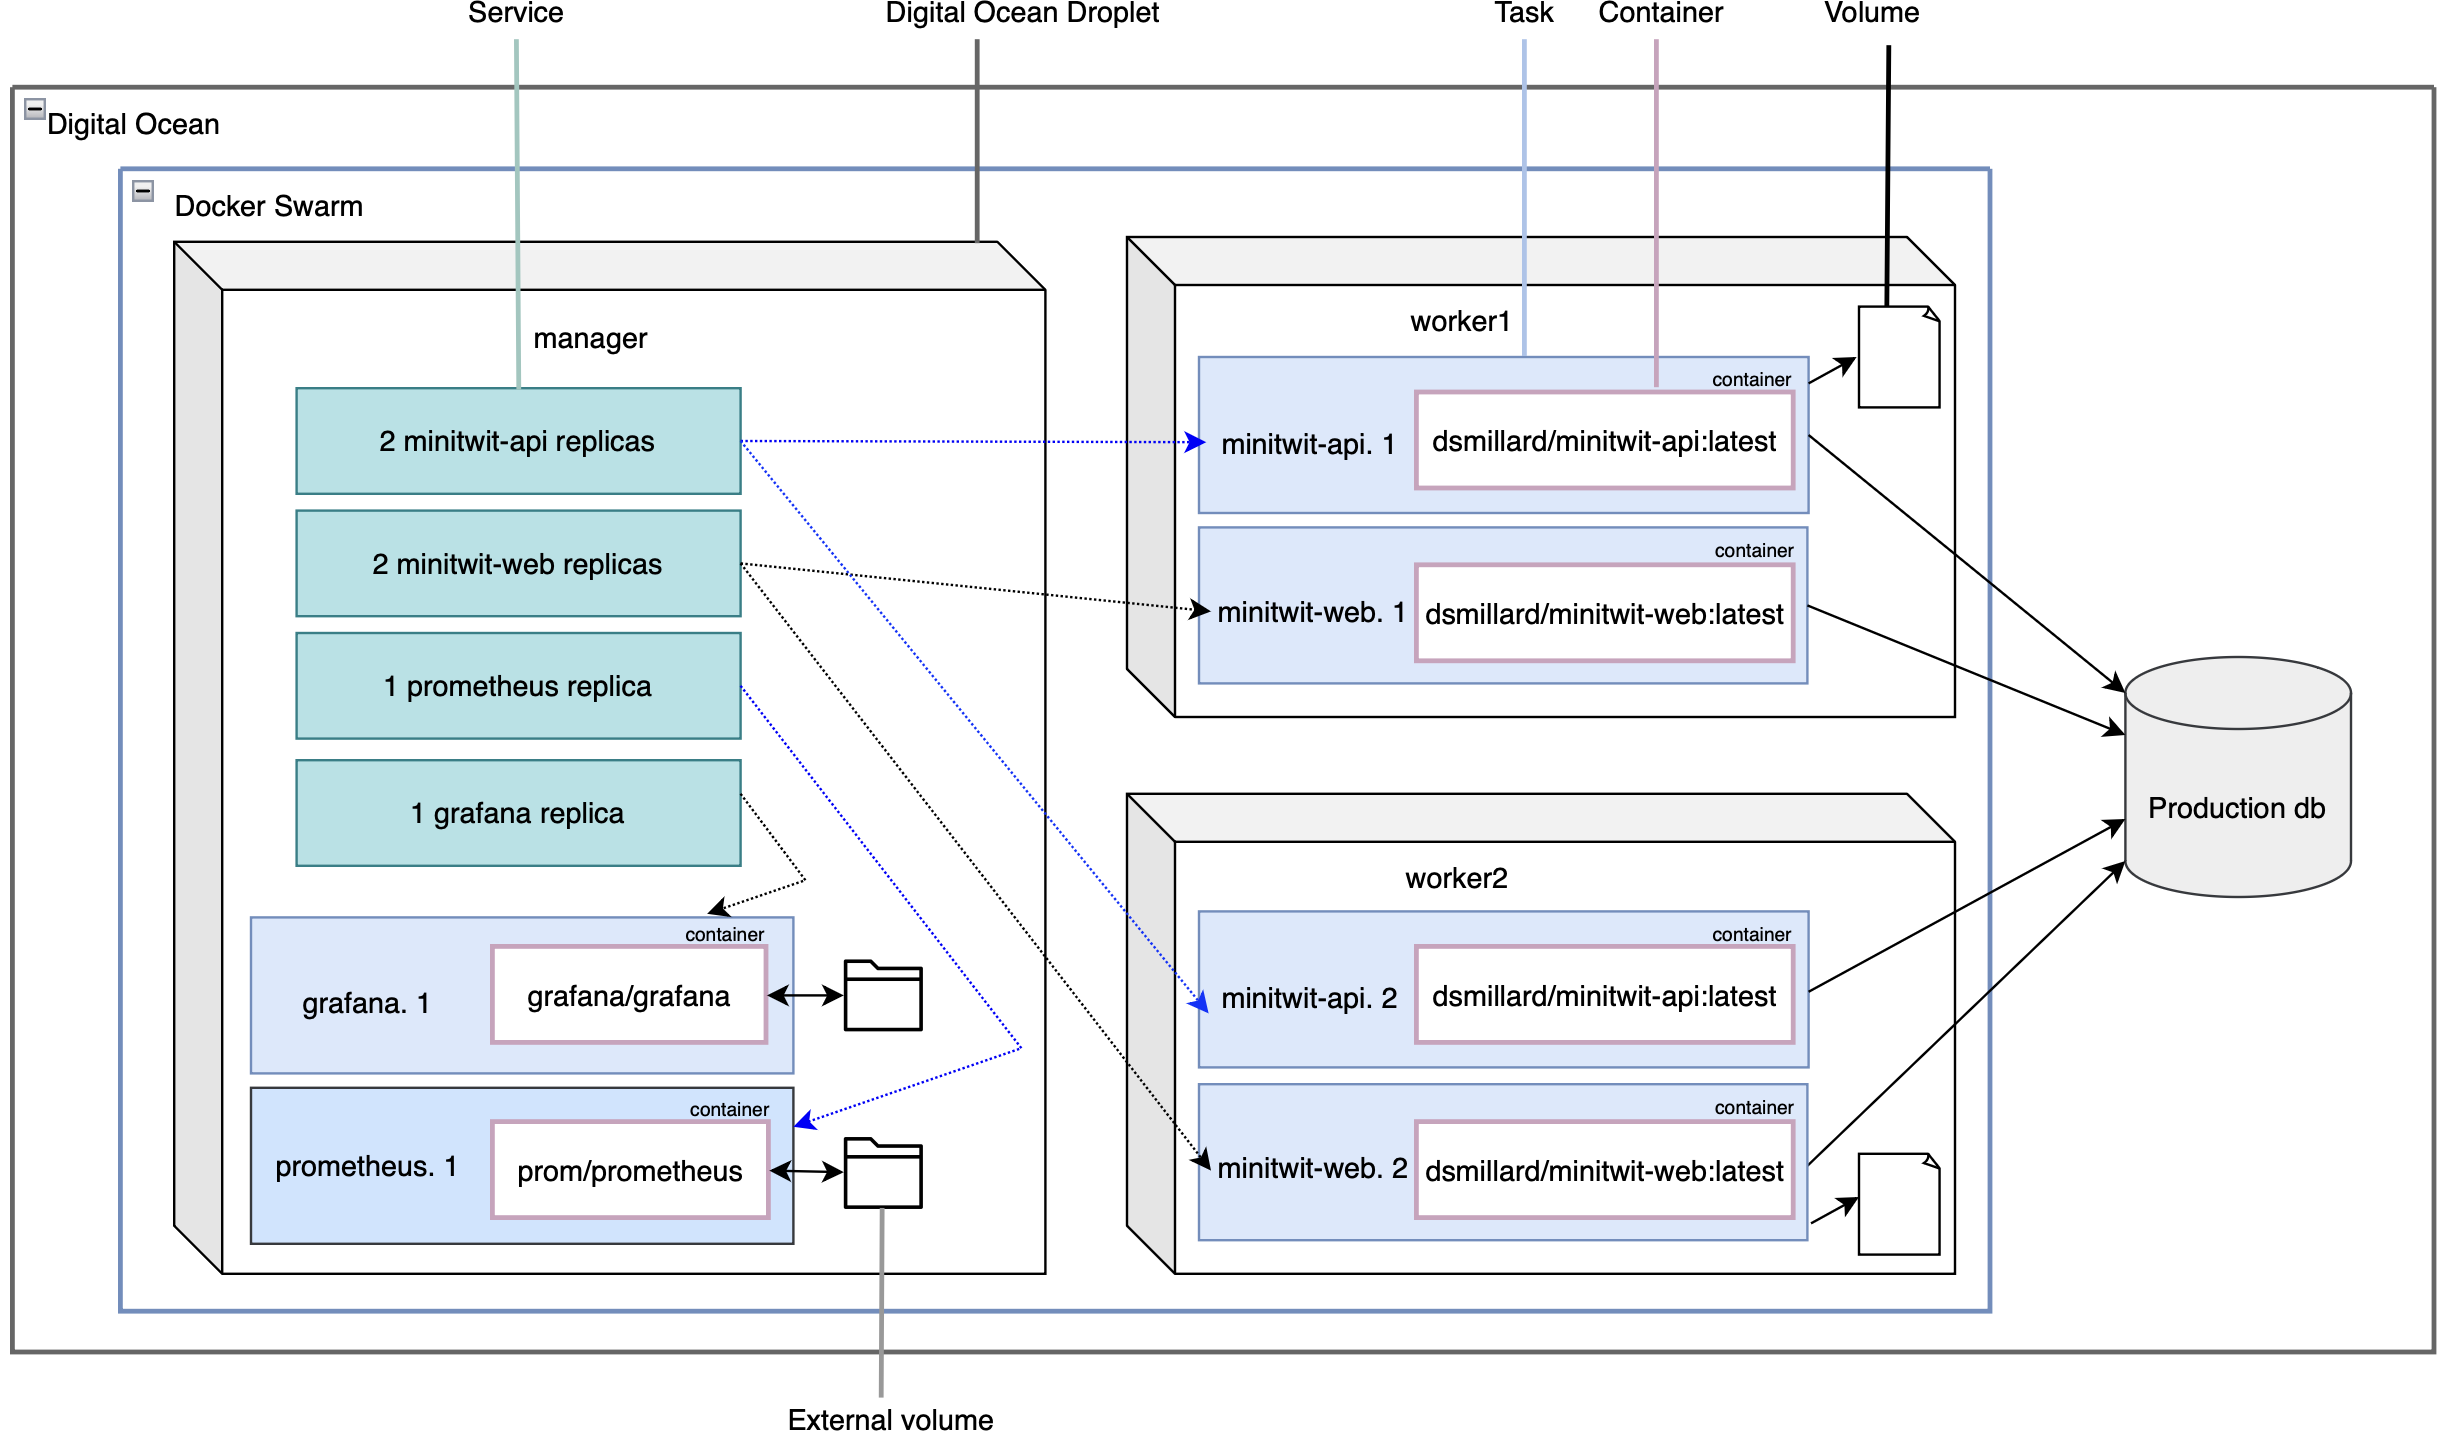
\includegraphics[width=\textwidth]{Images/docker_swarm.png}
  \caption{Docker Swarm service overview (coloring of the dotted lines are only for visibility).}
  \label{fig:dashboard}
\end{figure}
\subsubsection*{Ansible}
We have set up Ansible for Infrastructure as Code to create and configure droplets, then initialize and couple them together into a Docker Swarm. Although it should be usable in production, we currently only use Personal Access Tokens (PATs) from other Digital Ocean projects, to use them as test environment for infrastructural changes. \\

Our first Ansible playbook, "create droplets," uses a Digital Ocean PAT and a fingerprint to create three droplets. Based on their IP addresses and names, it auto-generates an inventory.ini file using a Jinja2 template. This inventory file allows us to run tasks for "all", "manager", or "workers". You can even limit tasks to a specific worker using the \texttt{--limit <hostname>} option. Additionally, the "create droplets" playbook includes a feature to delete the droplets and the inventory file by running it with the \texttt{--tags teardown} option.\\

Our second Ansible playbook, "configure\_swarm," uses the generated inventory file to configure the created droplets. It installs Docker and Docker Compose, opens necessary ports, syncs files, initializes a Docker Swarm on the manager and joins worker nodes to the Swarm.\\

We implemented these playbooks later in the project, which allowed us to experiment with our deployment scripts, droplet configurations, and Swarm setups in a test environment. Given additional time, we would have aimed to implement Ansible in production, automate the processes, and utilize it to develop a comprehensive restore strategy.

\begin{figure}[H]
  \centering
  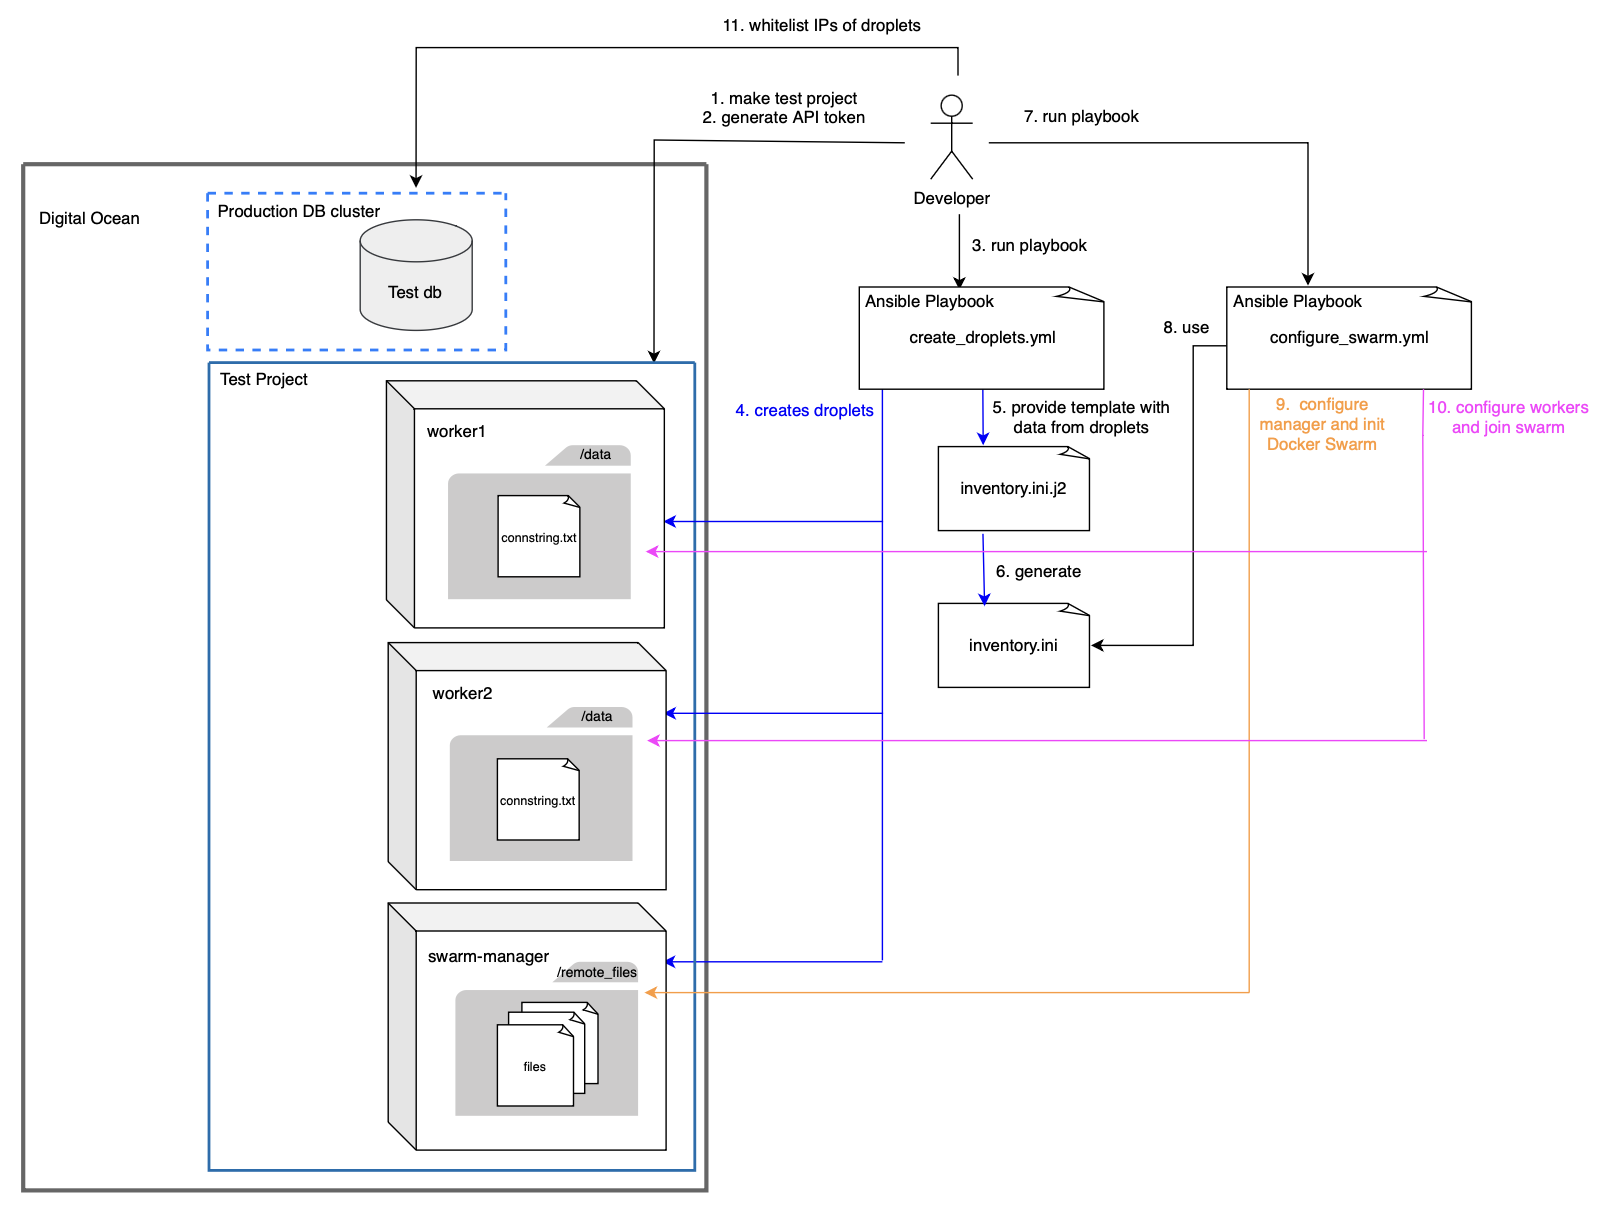
\includegraphics[width=\textwidth]{Images/ansible_setup.png}
  \caption{Our Ansible test environment setup, that initializes the docker swarm and makes sure that all droplets are configured with the right files and packages. It takes 2 minutes to create droplets and 2,5 minutes to configure the Swarm.}
  \label{fig:dashboard}
\end{figure}

\begin{figure}[H]
  \centering
  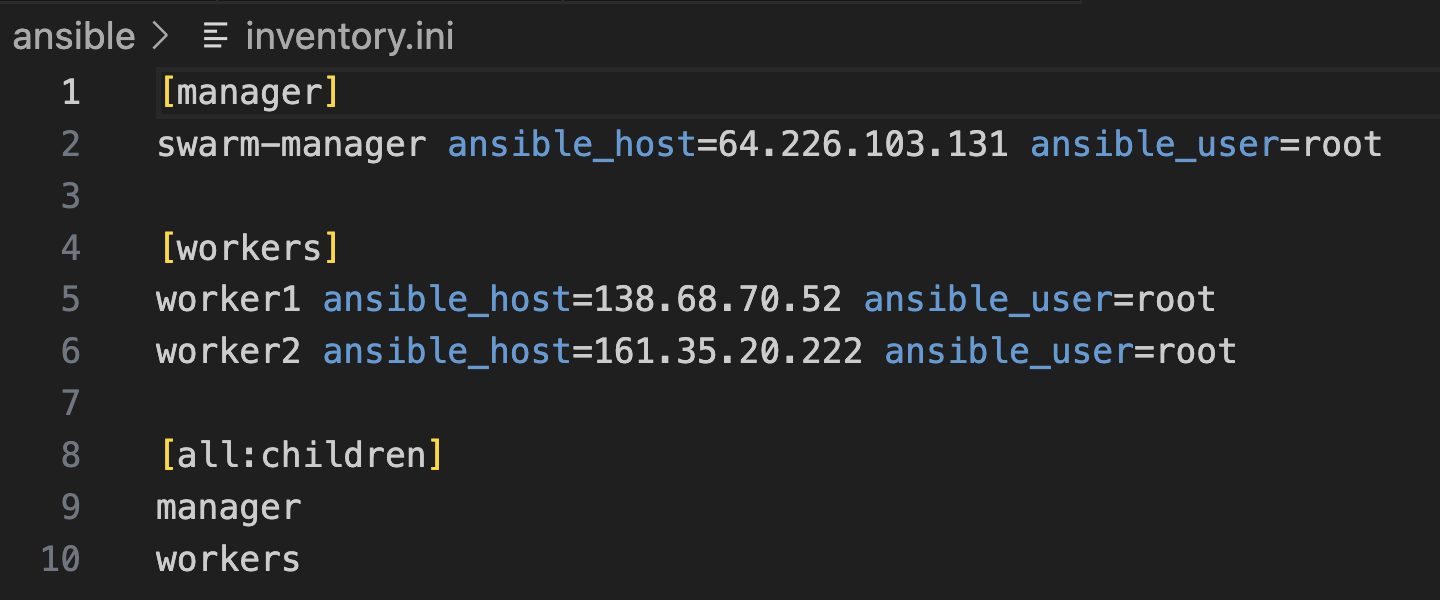
\includegraphics[width=\textwidth]{Images/ansible_inventory_file.png}
  \caption{Example of an auto-generated inventory file after setting test-project using Ansible.}
  \label{fig:dashboard}
\end{figure}

\subsection{Use of AI}
% In case you have used AI-assistants during your project briefly explain which system(s) you used during the project and reflect how it supported/hindered your process.
We have been assisted by Copilot. It was primarily used to help with LINQ in our infrastructure as it is easier to ask Copilot to create the query. It did, however, at times give queries that could be improved \textbf{a lot}, and when asking about it Copilot would go ahead and fix the issue. \\

Copilot was also been great at explaining certain things that we were either unsure of or did not know about, and it often times provided us with good auto completions that we could use (and modify to our liking). \\

Lastly, with us not knowing much about Grafana and Prometheus, Copilot provided great support in this helping us make our PromQL queries for our dashboards.